% !TEX root = ParticleFilter.tex
\section{Experimental Results\label{experiments}}

\subsection{Outline of the Experiments}

Recall that the aim of the paper is to \aim. By examining the error (i.e. the difference between the particle filter estimate of the system state and the pseudo-truth data) under different conditions, the paper will present some preliminary estimates of the potential for the use of particle filtering in real-time crowd simulation. In particular, the paper will estimate the minimum number of particles ($N_p$) that are needed to model a system that has a given number of agents ($N_a$). Although the dynamics of the model used here are simpler than those of more advanced crowd models, and hence the particle filter is tasked with an easier problem than it would have to solve in a real-world scenario, these experiments provide valuable insight into the general \textit{potential} of the method for crowd simulation.

It is well known that one of the main drawbacks with a particle filter is that the number of particles required can explode as the complexity of the system increases~\citep[e.g.][]{snyder_obstacles_2008, carrassi_data_2018}. In this system, the complexity of the model is determined by the number of agents. As outlined in Section~\ref{method}, randomness is introduced through agent interactions.  Therefore the fewer the number of agents, the smaller the chance of interactions occurring and the lower the complexity. As the number of agents increases,we find that the number of interactions increases exponentially (Figure~\ref{fig:collision_count}, discussed in the following section, will illustrate this). The paper will also experiment with the amount of particle noise that needs to be included to reduce the problem of particle deprivation ($\sigma_p$), but this is not a focus of the experiments.

%Figure~\ref{fig:PF_flowchart} outlined the modelling process. The particle filter runs in parallel to a single instance of the StationSim model, which is used to create pseudo-truth data (observations) representing the the locations of each agent at a given iteration. In each data assimilation `window', the truth model and all particles are stepped forward a number of iterations. At the end of the window the particle filter receives pseudo-true observations and uses these to calculate the particle weights (i.e. the error associated with each particle).  

To quantify the `success' of each parameter configuration -- i.e. the number of particles $N_p$ and amount of particle noise $\sigma_p$ that allow the particle filter to reliably represent a system of $N_a$ agents -- an estimate of the overall error associated with a particular particle filter configuration is required. There are a number of different ways that this error could be calculated. Here, we calculate the mean weight of each particle after resampling in every data assimilation window (the weights vary during an experiment because in early windows there are few agents and hence very little stochasticity so particle errors are low). Then we take the mean of these individual particle errors. In addition, because the results from an individual experiment can vary slightly, each particle configuration is executed a number of times, $M$, and the median error across experiments is calculated.

Formally if $\nu(t,j)$ is the error of particle $j$ in a data assimilation window $t$, and the total number of windows is $T$, then the total error of that particle filter configuration across $M$  experiments is: 
\begin{equation}
  E_{N_p,\sigma_p,N_a} =  {\rm median}_M \left( \sum_{j=1}^{N_p}  \frac{\sum_{t=1}^{T}\nu(t)}{T} \right)
\end{equation}
where $median_M()$ calculates the median over $M$ experiments.

In summary, the Table~\ref{tab:experiment_parameters} outlines the parameters that are used in the experiments. There are a number of other model and particle filter parameters that can vary, but ultimately these do not influence the results outlined here and are not experimented with. The parameters, and code, are available in full from the project repository \cite{stationsimgit}. 
% \begin{quote}\url{XXXX github url}\end{quote}

\begin{table*}[ht] \caption{Main parameters used in the experiments}
	\begin{center}
		\begin{tabular}{l l l } 
		    \hline Parameter & Symbol & Value / Range \\
			\hline
			Number of agents & $N_a$ & $[ 2, 40 ]$ \\
			Number of particles & $N_p$ & $[ 1, 10000 ]$ \\
			Particle noise & $\sigma_p $ & $[0.25, 0.5]$ \\
			Measurement noise & $\sigma_m$ &  $1.0$ \\
			Number of experiments (repetitions) & M & 20 \\
			Model iterations in each data assimilation window & - & 100 \\ 
			\hline
	\end{tabular} \end{center} \label{tab:experiment_parameters}
\end{table*}%



\subsection{Results}

\subsubsection{Overall Error}

Figure~\ref{fig:median_abs_error} plots the median of the mean error over all experiments to show how it varies with differing numbers of agents and particles. Due to the computational difficulty in running experiments with large numbers of particles and the need for an exponential increase in the number of particles with the number of agents (discussed in detail below), there are fewer experiments with large numbers of particles and hence the the experiments are not distributed evenly across the agents/particles space. Thus the error is presented in the form of an interpolated heat map. Broadly there is a reduction in error from the bottom-right corner (few particles, many agents) to the top left corner (many particles, few agents). The results illustrate that, as expected, there is a larger error with increasing numbers of agents but this can be mediated with larger numbers of particles. Note the logarithmic scale used on the vertical axis; an exponentially greater number of particles is required for each additional agent included in the simulation. 

\begin{figure}[ht]
	\centering
	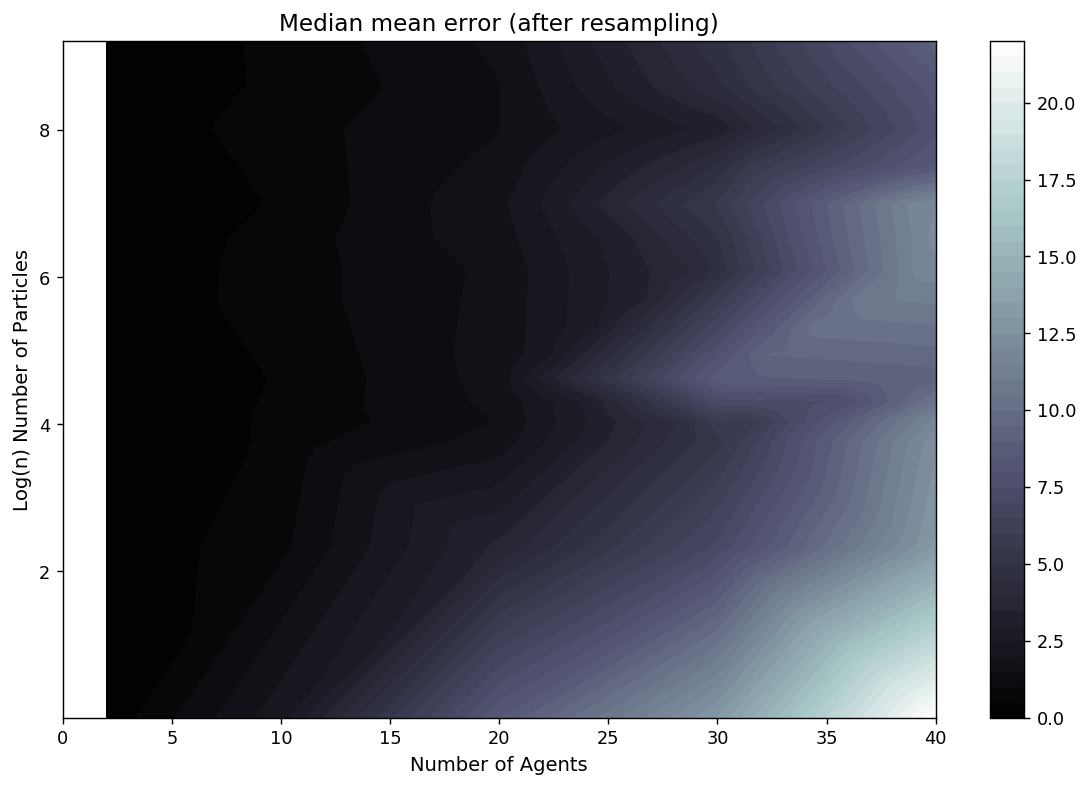
\includegraphics[width=0.7\textwidth]{figures/results/median_abs_error}
	\caption{Median of the mean errors after resampling} \label{fig:median_abs_error}
\end{figure}

There are two reasons for this exponential increase in the number of particles required. Firstly, as the number of agents increases so does the dimensionality of the state space. Also, and perhaps more importantly, with additional agents the chances of collisions, and hence stochastic behaviour, increases exponentially. This is illustrated by Figure~\ref{fig:collision_count} which presents the total number of collisions that occur across a number of simulations with a given number of agents.

\begin{figure}[ht]
	\centering
	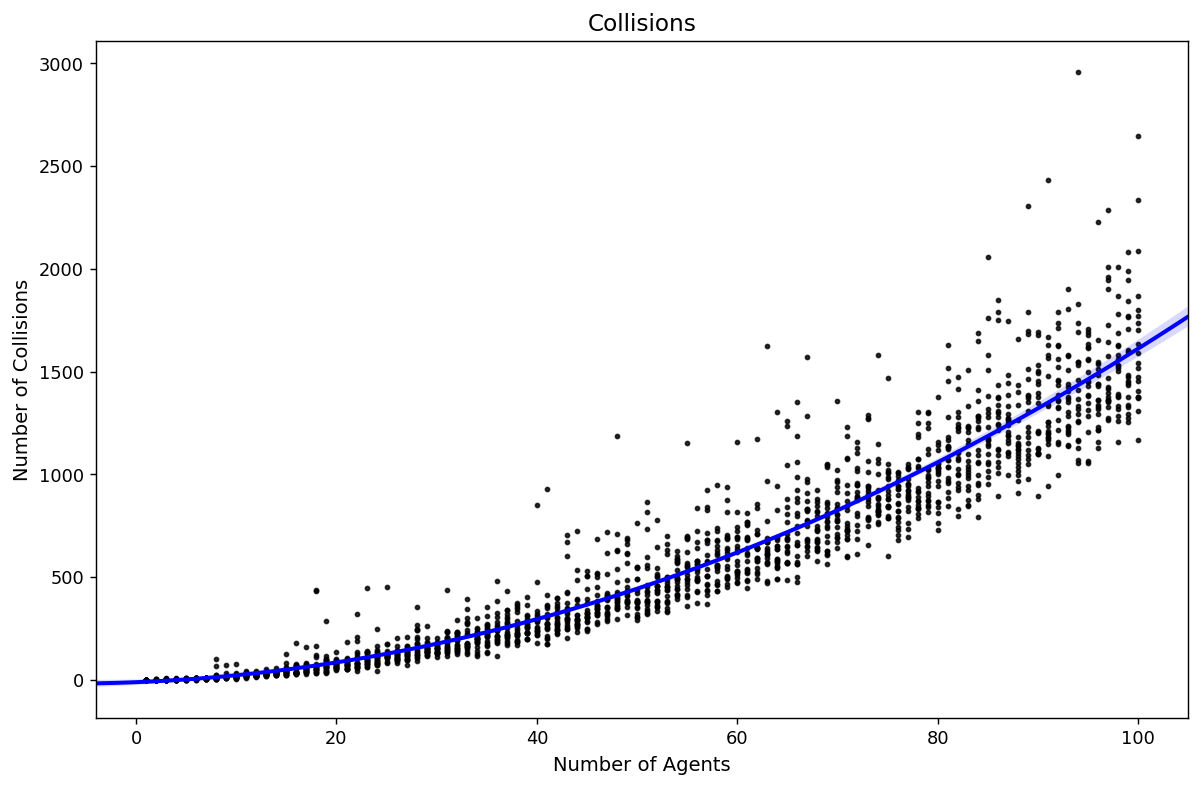
\includegraphics[width=0.7\textwidth]{figures/results/wiggle_count}
	\caption{The total number of collisions that occur given the number of agents. The blue line represents a polynomial regression model of order 2 with 99\% confidence intervals.} \label{fig:collision_count}
\end{figure}

On its own, the overall particle filter error (Figure~\ref{fig:median_abs_error}) reveals little information about which configurations would be judged `sufficiently reliable' to be used in practice. Therefore it is illuminating to visualise some of the results of individual particle filter runs to see how the estimates of the individual agents' locations vary, and what might be considered an `acceptable' estimate of the true state. Figure~\ref{fig:ani-10agents-10particles} illustrates the state of a particle filter with 10 particles and 10 agents at the end of its first data assimilation window (after resampling). With only ten agents in the system there are few, if any, collisions and hence very little stochasticity; all particles are able to represent the locations of the agents accurately.

\begin{figure}[ht]
	\centering
	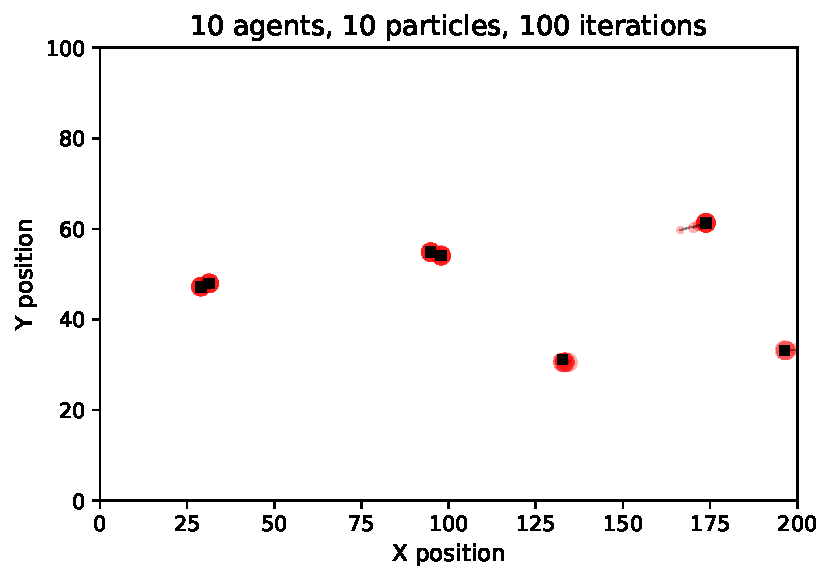
\includegraphics[width=0.45\textwidth]{figures/results/ani-10agents-10particles-window100}
	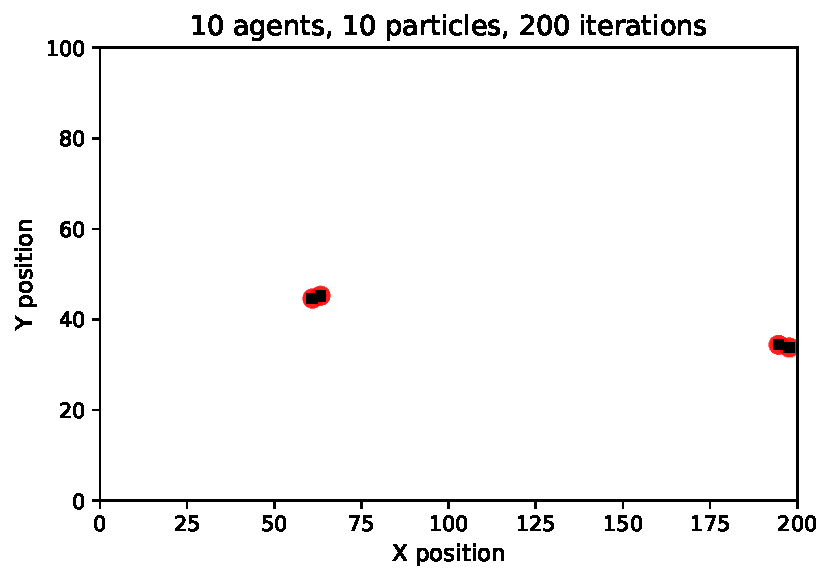
\includegraphics[width=0.45\textwidth]{figures/results/ani-10agents-10particles-window200}
	\caption{State of a particle filter with 10 agents and 10 particles after 100 and 200 iterations (after resampling at the end of the first and second data assimilation windows). Black squares illustrate the (pseudo) real locations of the agents and red circles represent the locations of those agents as predicted by individual particles (in this case all particles predict the agents' locations accurately and hence the red circles overlap).} \label{fig:ani-10agents-10particles}
\end{figure}

As the number of agents increases, collisions become much more likely and the chance of a particle diverging from the pseudo-truth state increases considerably. It becomes more common that no single particle will correctly capture the behaviours of \textit{all} agents. Therefore even after resampling there are some agents whose locations the particle filter is not able to accurately represent. Figure~\ref{fig:ani-50agents-10particles} illustrates a filter running with 40 agents and still only 10 particles. The long black lines show the locations of pseudo-real agents and the corresponding agents in the individual particles; it is clear that for some agents none of the particles have captured their pseudo-real locations. This problem can be mediated by increasing the number of particles. Figure~\ref{fig:median_abs_error} showed that with approximately 10,000 particles the error for simulations with 40 agents drops to levels that are comparable to the simulations of 10 agents. Hence a rule of thumb is that any particle filter with an overall error that is comparable to a clearly successful filter (i.e. Figure~\ref{fig:ani-10agents-10particles}) are reliably estimating the state of the system.

\begin{figure}[ht]
	\centering
	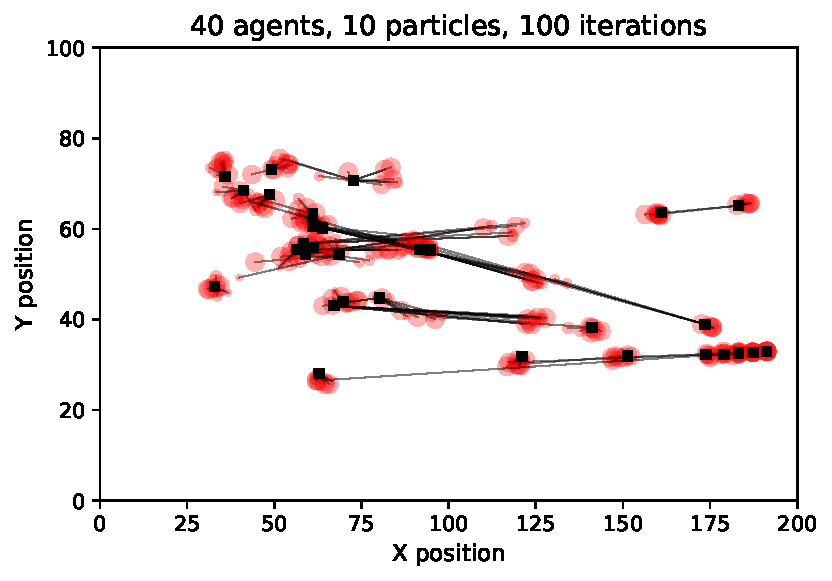
\includegraphics[width=0.45\textwidth]{figures/results/ani-40agents-10particles-window100}
	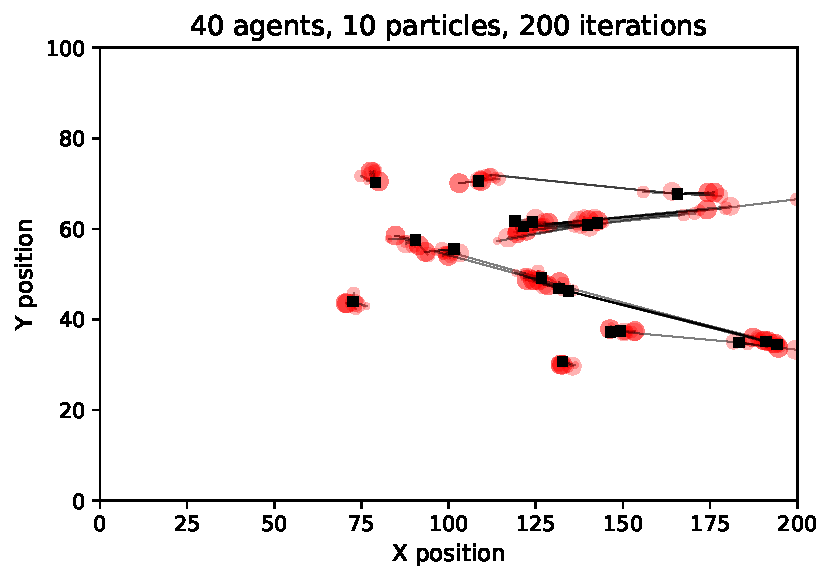
\includegraphics[width=0.45\textwidth]{figures/results/ani-40agents-10particles-window200}
	\caption{State of a particle filter with 50 agents and 10 particles. Lines connecting black squares (the pseudo-real agent locations) to red circles (particle estimate of the agent location) show that some particle estimates are a long way from the true agent locations.} \label{fig:ani-50agents-10particles}
\end{figure}



\subsubsection{Impact of Resampling}

Resampling is the process of weighting all particles according to how well they represent the pseudo-truth data; those with higher weights are more likely to be sampled and used in the following data assimilation window. This is important to analyse because it is the means by which the particle filter improves the overall quality of its estimates. Figure~\ref{fig:resampling} illustrates the impact of resampling on the error of the particle filter. With fewer than 10 agents in the system resampling is unnecessary because all particles are able to successfully model the state of the system. With more than 10 agents, however, it becomes clear that the population of particles will rapidly diverge from the pseudo-truth system state and resampling is essential for the filter manage to limit the overall error.

\begin{figure}[ht]
	\centering
	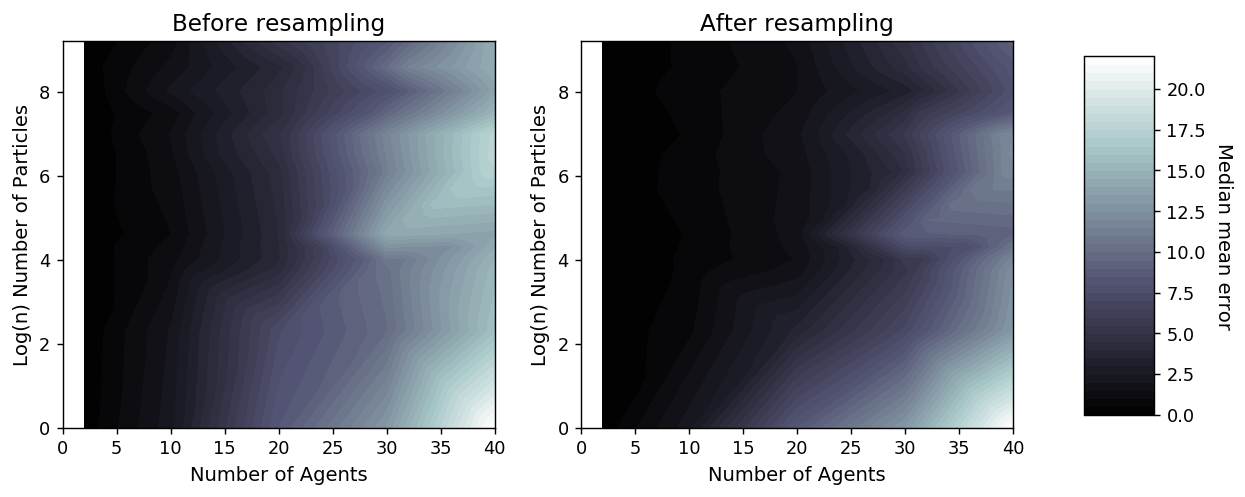
\includegraphics[width=0.9\textwidth]{figures/results/resampling}
	\caption{Median of the mean errors before and after resampling}\label{fig:resampling}
\end{figure}

\subsubsection{Particle Variance}

As discussed in Section~\ref{particle_sampling}, the variance of the population of particles can be a reliable measure for estimating whether particle deprivation is occurring. If there is very little variance in the particles, then it is likely that they have converged close to a single point in the space of possible states. This needs to be avoided because, in such situations, it is extremely unlikely that any particles will reliably represent the state of the real system. Figure~\ref{fig:variance_results} illustrates this by visualising the mean error of all particles, $\nu(t)$ (defined in Equation~\ref{eqn:particle_error}), in each data assimilation window, $t$, and their variance under different numbers of agents and particles. Note that each agent/particle configuration is executed 10 times and the results are visualised as boxplots. Also, simulations with larger numbers of agents are likely to run for a larger number of iterations, but the long-running models usually have very few agents in them in later iterations (most have left, leaving only a few slow agents). Hence only errors up to 600 iterations, where most of the agents have left the environment in most of the simulations, are shown. The graphs in Figure~\ref{fig:variance_results} can be interpreted as follows: 

\begin{figure}[ht]
	\centering
	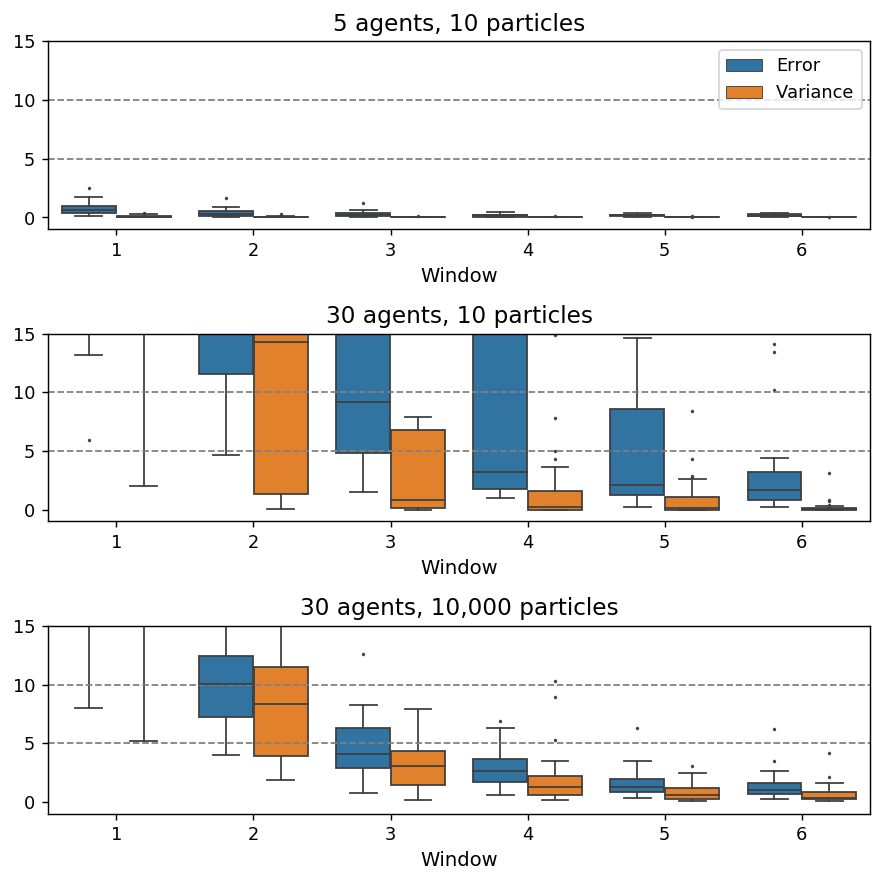
\includegraphics[width=0.9\textwidth]{figures/results/variance_results}
	\caption{Mean error and variance of particles under different combinations of the number of particles and number of agents}\label{fig:variance_results}
\end{figure}

\begin{itemize}
    \item With \textbf{5 agents and 10 particles} there is very low error and low variance (so low that the box plots are difficult to make out on Figure~\ref{fig:variance_results}). This suggests that particle deprivation is occurring, but there are so few agents that the simulation is largely deterministic so the particles are likely to simulate the pseudo-truth observations accurately regardless.
    \item When the number of agents is increased to \textbf{30 agents and 10 particles}, the errors are much larger. The increased non-linearity introduced by the greater number of agents (and hence greater number of collisions) means that the population of particles, as a whole, is not able to simulate the pseudo-truth data. Although particle variance can be high, none of the particles are successfully simulating the target.
    \item Finally, with \textbf{30 agents and 10,000 particles}, the errors are relatively low in comparison, especially after the first few data assimilation windows. 
\end{itemize}




\subsubsection{Particle Noise}

The number of particles ($N_p$) is the most important hyper-parameter, but the amount of noise added to the particles ($\sigma_p$) is also important as this is the means by which particle deprivation is prevented. However, the addition of too much noise will push a particle a long way away from the true underlying state. Under these circumstances, although particle deprivation is unlikely none of the particles will be close to the true state. To illustrate this, Figure~\ref{fig:median_abs_error-noise2.0} presents the median error with a greater amount of noise ($\sigma_p=0.5$). The overall pattern is similar to the equivalent graph produced with $\sigma_p=0.25$ in Figure~\ref{fig:median_abs_error} -- as the number of agents in the simulation ($N_a$) increases so does the number of particles required to maintain low error ($N_p$)  -- but the overall error in each $N_a$/$N_p$ combination is substantially larger for the experiments with additional noise. Future work could explore the optimal amount of noise in more detail; $\sigma=0.25$ was found to be the most reliable through trial and error.

\begin{figure}[ht]
	\centering
	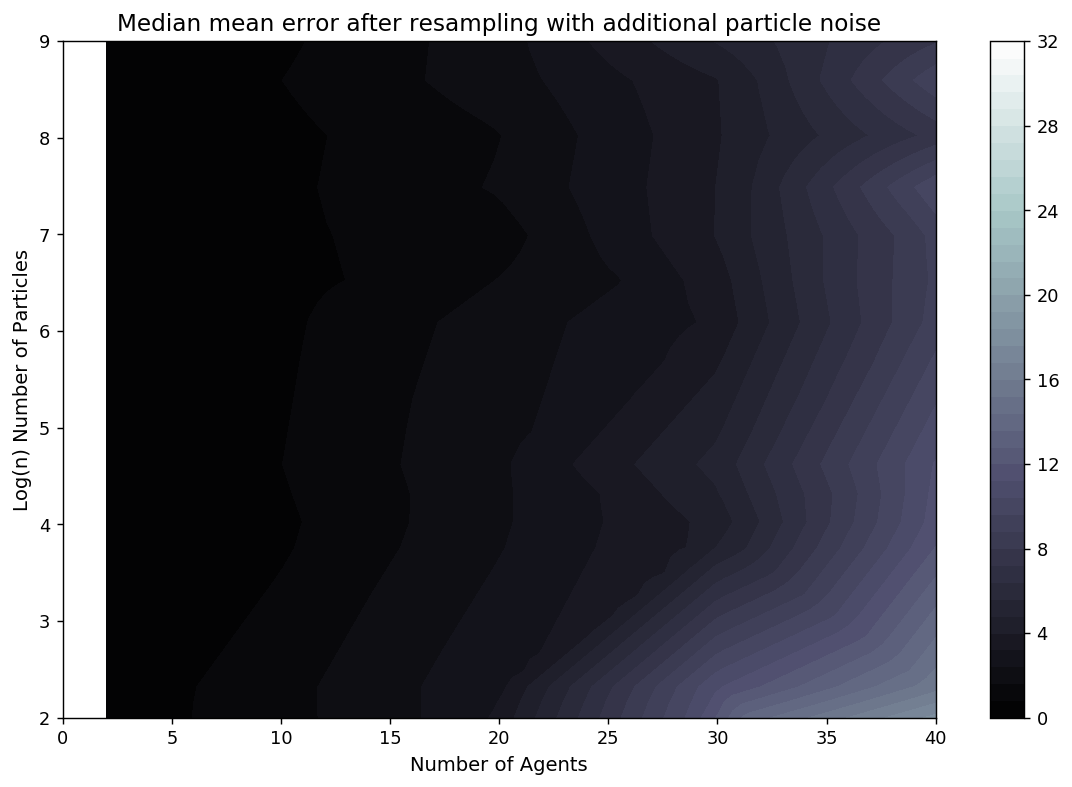
\includegraphics[width=0.5\textwidth]{figures/results/median_abs_error-noise2_0}
	\caption{Median of the mean errors after resampling with additional noise ($\sigma=0.5$).} \label{fig:median_abs_error-noise2.0}
\end{figure}

